\section{Setup - Step by step}
Building the project from nothing can be a quite involved process. Reserve plenty of time and prepare a cup of tea. 

\subsection{Getting started}
To get started with the PYNQ one must first set it up properly and hook it up to a computer. Start by following this guide:\\
\url{https://pynq.readthedocs.io/en/latest/getting_started.html}

\subsection{Installing dependencies}
If the latest PYNQ image (\ref{vSoftware}) is used, all of the dependencies used in the project come pre-installed.

However, if for some reason OpenCV for Python or Numpy are unavailable, it is highly recommended that you hook the PYNQ up to an Internet connection in order to download the dependencies easily.

\subsection{Development environment}
On your development computer you will need to install Vivado 2018.2 to continue development. This can be downloaded from here: \url{https://www.xilinx.com/support/download.html}. And good luck.

\subsection{Scala and Chisel 3 Modules}\label{ScalaChiselSub}
The accelerator modules are written using Chisel 3. You will first need to set up Chisel 3 and Scala. Follow the guide in the Chisel repository: \url{https://github.com/freechipsproject/chisel3}.

To be able to add your Chisel module into the Vivado project you need to compile the Chisel code into Verilog. The Verilog files will be imported into the Vivado project when it is created.

\subsection{Loading project into Vivado}
In the BRICOLEUR GitHub repository you will find a \texttt{pipeline.tcl} file that you will need to import our modules into the Vivado project. The rough outline below will demonstrate how this is set up:

\begin{itemize}
    \item Start Vivado 2018.2
    \item Create a new RTL project
    \item During the wizard it will ask for a set of source files, which are the Verilog files compiled in \ref{ScalaChiselSub}.
    \item After creating the project, go into the Tools menu and click \texttt{Run TCL Script} and locate the aforementioned \texttt{pipeline.tcl} file.
    \item Make sure to set the correct project constraints compatible with the PYNQ.
\end{itemize}

\subsection{Exporting Vivado project}
When you have added your new module to the project and connected your module in the block design you can generate the bitstream. Press \texttt{Generate bitstream} and \underline{\underline{wait}}.

When the bitstream is created you are ready to export it for execution on the PYNQ. Click on \texttt{File} and then \texttt{Export bitstream} and save it somewhere. You will now have to transfer this file onto the PYNQ to be utilized within the Python environment.

\subsection{Run on the PYNQ}
Run the python script on the PYNQ system and make sure to import your newly updated bitstream.

To upload to the PYNQ, run these commands:
\lstset{basicstyle=\small}
\begin{lstlisting}[language=bash]
scp <pathToBitstream>/design.bit xilinx@192.168.2.99:/home/xilinx/
scp <pathToTclScript>/design.tcl xilinx@192.168.2.99:/home/xilinx/
\end{lstlisting}

\subsection{Preparing the BRICOLEUR PCB}

\subsubsection{Programming the MCU}
You will need: 

\begin{itemize}
    \item 1 USB-UART device + USB cable
    \item Female-female jumper cables
    \item A way to supply power to the board (USB-micro cable/PYNQ board)
\end{itemize}

The EFM32GG980 can be programmed using the bootloader which comes pre-installed on the chip. Compile the MCU code to produce the desired \texttt{.bin} file. Depending on your method of development, make sure that the loader sets a base offset of 0x4000, to respect the bootloader's space. Also reduce the available flash memory accordingly. Then prepare the PCB for flashing. 
\begin{enumerate}
    \item Connect the USB-UART device to your computer, make sure it works. 
    \item Connect the UART device to the UART\_BOOT port, between the MCU and the logo, on the PCB. Pin 6 should be connected to RX, and pin 4 to TX.
    \item Using a jumper, connect pin 9 on the PCB debug connector (top left corner) to pin 1 (VMCU). This enables launch to bootloader instead of an existing program.
    \item Connect a power source to the PCB. 
    \item Launch your serial communication program of choice, such as Screen, MiniCom or Putty. 
    \item Push the reset button, located closest to the MCU. 
    \item Quickly send the character 'U' to initialize bootloader communication. 
    \item Then send 'u' to perform a non-destructive upload. 
    \item Using Xmodem-CRC, transfer the binary. In 'screen' this would be done by pressing Ctrl-a, followed by ':', and the command: 
    \lstset{basicstyle=\small}
    \begin{lstlisting}[language=bash]
        exec !! sx bricoleur.bin
    \end{lstlisting}
    \item Verify that the program runs as expected by sending 'b'. 
\end{enumerate}

\subsection{Putting everything together}

\begin{wrapfigure}{R}{0.4\textwidth}
    \centering
    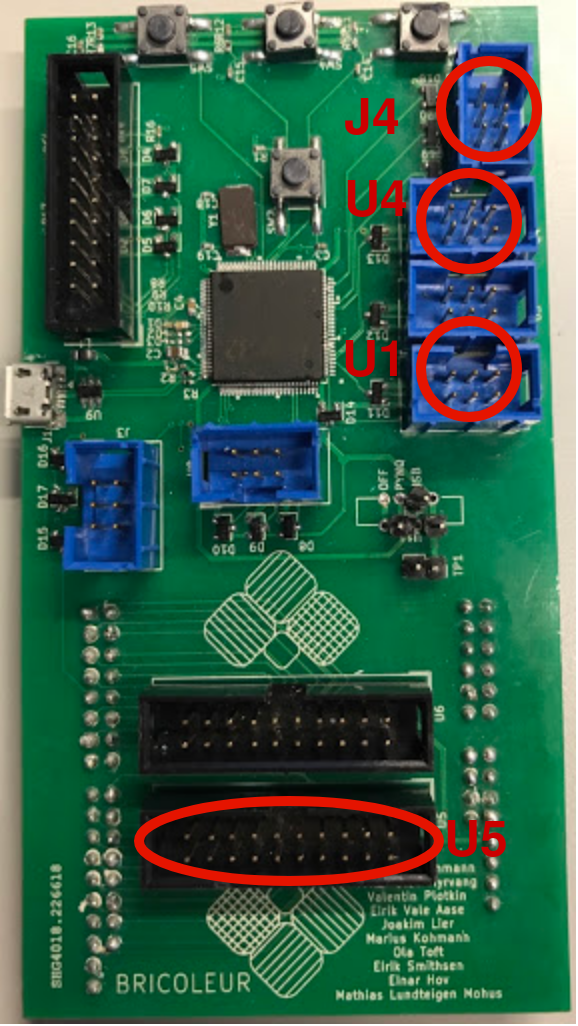
\includegraphics[scale=0.2]{Images/PCB_CONN.png}
    \caption{Connections for basic functionality}
    \label{fig:pcb_connections}
\end{wrapfigure}

Assemble the boards as shown on the image. The BRICOLEUR system can be configured in multiple ways. However, in order to reproduce the demo-build, connect it as follows:

\begin{enumerate}
    \item Connect U1 to the left ultrasonic sensor, and U4 to the right one. 
    \item Connect the top right IDC (J4) to an external unit. 
    \item \sout{Connect the OV5642 camera to U5.} Connect the ethernet cable to the PYNQ instead. 
    \item Connect a jumper or physical switch to the desired power source pin, in this case the PYNQ, and the VMCU pin (bottom left on  switch area).
    \item Put the PCB on top of the PYNQ by joining the matching headers.
\end{enumerate}

%Clearpage is here to prevent wrapfigure fuckup, since the PCB figure wraps on the section under, preventing the ultrasound placement figure to wrap this section (for some reason, i guess Overleaf doesn't like wrapping on the same section of text)
\clearpage

\subsubsection{Sensor placement}

\begin{wrapfigure}{R}{0.31\textwidth}
    \centering
    
\includegraphics[scale=0.25]{Images/Ultra_Distance.png}
    \caption{Things to consider when placing sensors}
    \label{fig:ultra_dist}
\end{wrapfigure}

The positioning of the ultrasonic sensors is based on two main variables: Area of overlap and distance between the sensors. Both should be maximised to achieve the best results.

A larger area of overlap means there is a larger area where both sensors will detect the object, and therefore be able to do meaningful calculations. A larger distance \texttt{D} between the sensors gives a larger difference in the distance from each sensor to object \texttt{O}. This in turn makes it easier to calculate an accurate X-coordinate of the object, but it also lowers the area of overlap.

The demo build chose a distance of 30.5 cm.
